\documentclass{beamer}
\mode<presentation>
\usepackage{amsmath}
\usepackage{amssymb}
%\usepackage{advdate}
\usepackage{adjustbox}
\usepackage{subcaption}
\usepackage{enumitem}
\usepackage{multicol}
\usepackage{mathtools}
\usepackage{listings}
\usepackage{float}
\usepackage{graphicx}
\usepackage{url}
\def\UrlBreaks{\do\/\do-}
\usetheme{Boadilla}
\usecolortheme{lily}
\setbeamertemplate{footline}
{
  \leavevmode%
  \hbox{%
  \begin{beamercolorbox}[wd=\paperwidth,ht=2.25ex,dp=1ex,right]{author in head/foot}%
    \insertframenumber{} / \inserttotalframenumber\hspace*{2ex} 
  \end{beamercolorbox}}%
  \vskip0pt%
}
\setbeamertemplate{navigation symbols}{}

\providecommand{\nCr}[2]{\,^{#1}C_{#2}} % nCr
\providecommand{\nPr}[2]{\,^{#1}P_{#2}} % nPr
\providecommand{\mbf}{\mathbf}
\providecommand{\pr}[1]{\ensuremath{\Pr\left(#1\right)}}
\providecommand{\qfunc}[1]{\ensuremath{Q\left(#1\right)}}
\providecommand{\sbrak}[1]{\ensuremath{{}\left[#1\right]}}
\providecommand{\lsbrak}[1]{\ensuremath{{}\left[#1\right.}}
\providecommand{\rsbrak}[1]{\ensuremath{{}\left.#1\right]}}
\providecommand{\brak}[1]{\ensuremath{\left(#1\right)}}
\providecommand{\lbrak}[1]{\ensuremath{\left(#1\right.}}
\providecommand{\rbrak}[1]{\ensuremath{\left.#1\right)}}
\providecommand{\cbrak}[1]{\ensuremath{\left\{#1\right\}}}
\providecommand{\lcbrak}[1]{\ensuremath{\left\{#1\right.}}
\providecommand{\rcbrak}[1]{\ensuremath{\left.#1\right\}}}
\theoremstyle{remark}
\newtheorem{rem}{Remark}
\newcommand{\sgn}{\mathop{\mathrm{sgn}}}
\providecommand{\abs}[1]{\left\vert#1\right\vert}
\providecommand{\res}[1]{\Res\displaylimits_{#1}} 
\providecommand{\norm}[1]{\lVert#1\rVert}
\providecommand{\mtx}[1]{\mathbf{#1}}
\providecommand{\mean}[1]{E\left[ #1 \right]}
\providecommand{\fourier}{\overset{\mathcal{F}}{ \rightleftharpoons}}
%\providecommand{\hilbert}{\overset{\mathcal{H}}{ \rightleftharpoons}}
\providecommand{\system}{\overset{\mathcal{H}}{ \longleftrightarrow}}
	%\newcommand{\solution}[2]{\textbf{Solution:}{#1}}
%\newcommand{\solution}{\noindent \textbf{Solution: }}
\providecommand{\dec}[2]{\ensuremath{\overset{#1}{\underset{#2}{\gtrless}}}}
\newcommand{\myvec}[1]{\ensuremath{\begin{pmatrix}#1\end{pmatrix}}}
\let\vec\mathbf

\lstset{
language=C,
frame=single, 
breaklines=true,
columns=fullflexible
}

\numberwithin{equation}{section}

\title{Presentation - Matgeo}
\author{Aryansingh Sonaye \\
AI25BTECH11032 \\
EE1030 - Matrix Theory}

\date{\today} 
\begin{document}

\begin{frame}
\titlepage
\end{frame}

\section{Problem}
\begin{frame}
\frametitle{Problem Statement}
\textbf{Problem 7.3.5}

If a circle passes through the points $(0,0)$, $(a,0)$ and $(0,b)$, then find the coordinates of its centre.


\end{frame}

\section{Solution}
\subsection{Description of Variables used}
\begin{frame}
\frametitle{Description of Variables used}
\begin{table}[H]
\centering
\begin{tabular}{|c|c|}
\hline
Variable & Description \\
\hline
$\vec{x}_1 = \myvec{0 \\ 0}$ & First point on circle \\
\hline
$\vec{x}_2 = \myvec{a \\ 0}$ & Second point on circle \\
\hline
$\vec{x}_3 = \myvec{0 \\ b}$ & Third point on circle \\
\hline
\end{tabular}
\end{table}


\end{frame}

\subsection{Theoretical Solution }
\begin{frame}
\frametitle{Theoretical Solution}
From (7.1.3.1), for three points $\vec{x}_1, \vec{x}_2, \vec{x}_3$ on a circle:
\begin{align}
\myvec{
2\vec{x}_1 & 2\vec{x}_2 & 2\vec{x}_3 \\
1 & 1 & 1
}^\top
\myvec{\vec{u} \\ f}
=
-\myvec{\|\vec{x}_1\|^2 \\ \|\vec{x}_2\|^2 \\ \|\vec{x}_3\|^2},
\quad
\vec{c} = -\vec{u}.
\end{align}

Substituting the given points:
\begin{align}
\myvec{
0 & 2a & 0 \\
0 & 0 & 2b \\
1 & 1 & 1
}^\top
\myvec{u_1 \\ u_2 \\ f}
=
-\myvec{0 \\ a^2 \\ b^2}.
\end{align}

\end{frame}

\begin{frame}
\frametitle{Theoretical Solution}
This expands to:
\begin{align}
f &= 0, \\
2au_1 + a^2 &= 0, \\
2bu_2 + b^2 &= 0.
\end{align}

Solving:
\begin{align}
u_1 &= -\frac{a}{2}, \quad
u_2 = -\frac{b}{2}, \quad
f = 0.
\end{align}

Hence, the centre of the circle is
\begin{align}
\vec{c} = -\vec{u} = \myvec{\tfrac{a}{2} \\ \tfrac{b}{2}}.
\end{align}

\begin{align}
\boxed{\text{Centre of the circle is } \left(\tfrac{a}{2}, \tfrac{b}{2}\right)}
\end{align}

\end{frame}


\subsection{Plot}
\begin{frame}
    \frametitle{Plot}
\begin{figure}[H]
   \centering
   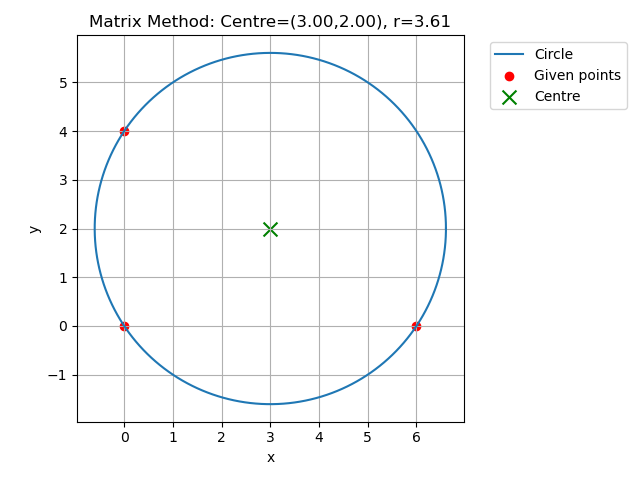
\includegraphics[width=0.8\columnwidth]{figs/newcentre.png}
   \caption{}
   \label{}
   \end{figure}
\end{frame}

\begin{frame}[fragile]
    \frametitle{Code - C}
    \begin{lstlisting}
#include <math.h>

// Circle through (0,0), (a,0), (0,b) using direct expansion of matrix equations
void circle_center_matrix(double a, double b,
                          double *cx, double *cy, double *r)
{
    // From equations:
    // f = 0
    // 2a u1 + f = -a^2  -> u1 = -a/2
    // 2b u2 + f = -b^2  -> u2 = -b/2
    double u1 = -a/2.0;
    double u2 = -b/2.0;

    *cx = -u1;   // = a/2
    *cy = -u2;   // = b/2



    \end{lstlisting}
    \end{frame}

    \begin{frame}[fragile]
    \frametitle{Code - C}
    \begin{lstlisting}
    if (r) {
        *r = sqrt((*cx)*(*cx) + (*cy)*(*cy));
    }
}




    \end{lstlisting}
    \end{frame}

\begin{frame}[fragile]
    \frametitle{Code - Python(with shared C code)}
    The code to obtain the required plot is
    \begin{lstlisting}
import ctypes as ct
import numpy as np
import matplotlib.pyplot as plt

# Load library
lib = ct.CDLL("./libcircle.so")

lib.circle_center_matrix.argtypes = [ct.c_double, ct.c_double,
                                     ct.POINTER(ct.c_double),
                                     ct.POINTER(ct.c_double),
                                     ct.POINTER(ct.c_double)]
lib.circle_center_matrix.restype = None

# Inputs
a, b = 6.0, 4.0
cx, cy, r = ct.c_double(), ct.c_double(), ct.c_double()


\end{lstlisting}
\end{frame}
\begin{frame}[fragile]
\frametitle{Code - Python(with shared C code)}
\begin{lstlisting}
lib.circle_center_matrix(a, b, ct.byref(cx), ct.byref(cy), ct.byref(r))
print(f"Centre = ({cx.value}, {cy.value}), Radius = {r.value}")
# Plot
theta = np.linspace(0, 2*np.pi, 400)
X = cx.value + r.value*np.cos(theta)
Y = cy.value + r.value*np.sin(theta)

plt.plot(X, Y, label="Circle")
plt.scatter([0,a,0], [0,0,b], color="red", label="Given points")
plt.scatter([cx.value], [cy.value], color="green", marker="x", s=100, label="Centre")
plt.gca().set_aspect("equal", adjustable="box")
plt.title(f"Direct Matrix Expansion: Centre=({cx.value:.2f},{cy.value:.2f}), r={r.value:.2f}")
plt.legend(); plt.grid(True)
plt.savefig("circle.png")
plt.show()


\end{lstlisting}
\end{frame}



\begin{frame}[fragile]
\frametitle{Code - Python only}
\begin{lstlisting}
# Circle through (0,0), (a,0), (0,b) using the matrix method
# Equation: ||x||^2 + 2u^T x + f = 0
# Centre = -u

import numpy as np
import matplotlib.pyplot as plt

# --- Input values ---
a = 6.0
b = 4.0

# --- Build the 3x3 system A [u1, u2, f]^T = b_vec ---
A = np.array([
    [0.0,   0.0, 1.0],
    [2.0*a, 0.0, 1.0],
    [0.0, 2.0*b, 1.0]
], dtype=float)



\end{lstlisting}
\end{frame}

\begin{frame}[fragile]
\frametitle{Code - Python only}
\begin{lstlisting}
b_vec = np.array([0.0, -a*a, -b*b], dtype=float)

# --- Solve for (u1, u2, f) ---
u1, u2, f = np.linalg.solve(A, b_vec)

# --- Centre and radius ---
cx, cy = -u1, -u2
r = np.hypot(cx, cy)

print(f"u = ({u1}, {u2}), f = {f}")
print(f"Centre = ({cx}, {cy})")
print(f"Radius = {r}")

# --- Plot the circle and points ---
theta = np.linspace(0, 2*np.pi, 400)
X = cx + r*np.cos(theta)
Y = cy + r*np.sin(theta)




\end{lstlisting}
\end{frame}

\begin{frame}[fragile]
\frametitle{Code - Python only}
\begin{lstlisting}
plt.figure()
plt.plot(X, Y, label="Circle")
plt.scatter([0, a, 0], [0, 0, b], color="red", label="Given points")
plt.scatter([cx], [cy], color="green", marker="x", s=100, label="Centre")
plt.gca().set_aspect("equal", adjustable="box")
plt.title(f"Matrix Method: Centre=({cx:.2f},{cy:.2f}), r={r:.2f}")
plt.xlabel("x"); plt.ylabel("y")
plt.grid(True)

# Place legend outside (right side)
plt.legend(loc="upper left", bbox_to_anchor=(1.05, 1.0))
plt.tight_layout()
plt.savefig("newcentre.png")
plt.show()



\end{lstlisting}
\end{frame}

\end{document}